% !TeX root = main.tex
% !TeX output_directory = ../out
\documentclass[journal,onecolumn]{IEEEtran}

\usepackage[utf8]{inputenc}
\usepackage[T1]{fontenc}
\usepackage{cite}
\usepackage{amsmath,amssymb,amsfonts}
\usepackage{graphicx}
\usepackage{tikz}
\usetikzlibrary{shapes.geometric, arrows, positioning}
\usepackage{hyperref}

\title{The Scriptorium Framework: A Scholarly Proposal for AI-Augmented Biblical Hermeneutics}
\author{Antigravity (Scholarly Assistant)}
\date{May 9, 2026}

\begin{document}

\maketitle

\begin{abstract}
Traditional Artificial Intelligence (AI) interactions in religious studies often suffer from "The Mirror Effect," where the model merely reflects back the user's input or provides low-level factual retrieval. This paper proposes the Scriptorium Framework, an advanced pedagogical model that transforms AI from a static repository into a Socratic Study Partner. By integrating the principles of Computational Hermeneutics with the Inductive Bible Study method and the Father-Child Relational Paradigm, the framework provides a "Value-Add" experience that stretches the user’s critical thinking and spiritual discernment beyond their own initial observations.
\end{abstract}


\section{Introduction}
The proliferation of Generative Artificial Intelligence (GenAI) has fundamentally altered the landscape of religious education and personal study. However, most existing AI tools function primarily as ``Search Engines with a Voice,'' providing deductive answers that often prematurely terminate the user's own reflective process. This phenomenon, which we term the ``Mirror Effect'' or ``Stochastic Parrot'' response \cite{bender2021parrots}, occurs when the AI reflects the user's cognitive biases or limits its feedback to a summary of the provided input, thereby offering zero ``Value-Add'' to the serious scholar.

\subsection{The Problem of Shallow Engagement}
The risks of AI in theological contexts extend beyond mere inaccuracy. As recent scholarship on AI in theological education warns, the ease of generating summaries and outlines may circumvent the ``formative struggle'' that is essential for intellectual and spiritual maturity. The process of wrestling with complex texts---what Ricoeur \cite{ricoeur1976} calls the ``surplus of meaning''---is itself the transformative act. When an AI short-circuits this struggle by providing a pre-digested answer, it robs the user of the very encounter that produces growth.

\subsection{Computational Hermeneutics}
To address these limitations, we draw upon the emerging field of Computational Hermeneutics \cite{kommers2026}. This discipline posits that AI should be used as an interpretive ``accelerator'' that navigates the situatedness and plural meanings of ancient texts. Rather than serving as an oracle, the AI acts as a mid-wife (\textit{maieutics}) to help the user give birth to new insights that were previously hidden by linguistic or cultural barriers. Gadamer's \cite{gadamer1960} concept of the ``fusion of horizons'' is instructive here: true understanding occurs not when the AI delivers a historical fact, but when the user's present-day ``horizon'' merges with the ancient text's ``horizon'' to produce a new, shared context of meaning.

\subsection{The Relational Disconnect}
A significant gap in contemporary Bible study literature is the ``Methodological Trap,'' where the study of sacred texts becomes a mechanical ritual of ``doing'' rather than ``relating'' \cite{packer1973}. Traditional Inductive Bible Study (IBS) methods, as formalized by Traina \cite{traina1952} and refined by Bauer and Traina \cite{bauer2011}, provide a rigorous three-step process of Observation, Interpretation, and Application (OIA). While invaluable, these methods can inadvertently lead to a ``checklist'' mentality that distances the reader from the Divine. In contrast, a relational hermeneutic rooted in the Father-Child paradigm suggests that the primary goal of the text is to facilitate a natural, spontaneous connection \cite{nih2024}. This paper proposes a framework that bridges this gap, using high-level computational tools to foster a child-like curiosity and intimacy.

\subsection{Paper Organization}
The remainder of this paper is organized as follows. Section 2 presents a gap analysis identifying the specific deficiencies in current AI-augmented Bible study tools. Section 3 establishes the theological foundation of the Relational Priority. Section 4 details the three-layer Scriptorium Cycle methodology. Section 5 specifies the implementation rules and discusses future research directions.


\section{The Relational Priority}
At the core of the Scriptorium Framework is the Father-Child Paradigm. In many contexts, Bible study devolves into a ritual of "methods for the sake of doing"—a mechanical checklist that can stifle intimacy. The framework enforces the principle that a child does not require a complex methodology to approach their father; relationship is natural and spontaneous.

\subsection{The AI's Relational Role}
The AI must never act as a "Taskmaster" or a "Method-Enforcer." Instead, all linguistic and historical tools are secondary to the goal of building the user's relationship with God. The AI facilitates a "Natural Conversation" with the text, encouraging the user to speak to God as a Father, ensuring that the study metric is intimacy rather than academic completion.


\section{Methodology: The Scriptorium Cycle}
The Scriptorium Framework operates through a recursive cycle consisting of three distinct layers of analysis \cite{schon1983}:

\begin{enumerate}
    \item \textbf{The Linguistic Scalpel:} Utilizing semantic domain analysis to uncover the root intensity of original languages (Greek/Hebrew).
    \item \textbf{The Historical-Critical Shock:} Grounding the text in its original socio-cultural and legal context \cite{malina2001}.
    \item \textbf{The Pauline Bridge:} Mapping relational roles (Advocate, Offender, Reconciler) to modern personal application \cite{hendricks1991}.
\end{enumerate}

\begin{figure}[htbp]
\centering
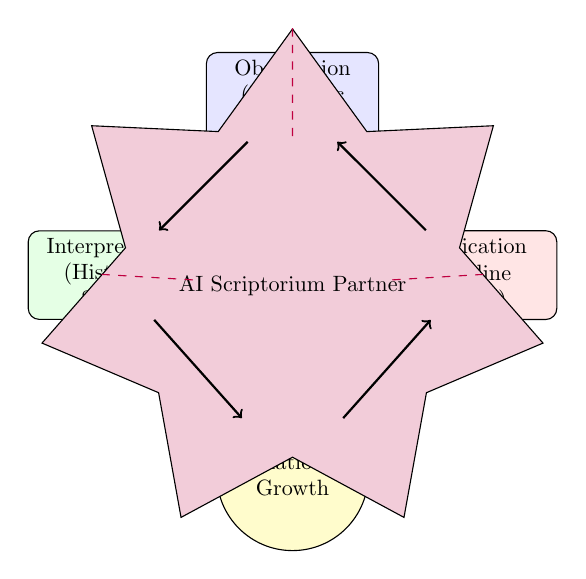
\begin{tikzpicture}[node distance=2cm, auto, scale=0.8, every node/.style={scale=0.8}]
    % Nodes
    \node (obs) [draw, rounded corners, fill=blue!10, text width=2.5cm, align=center] {Observation \\ (Linguistic Scalpel)};
    \node (int) [below left of=obs, node distance=4cm, draw, rounded corners, fill=green!10, text width=2.5cm, align=center] {Interpretation \\ (Historical Shock)};
    \node (app) [below right of=obs, node distance=4cm, draw, rounded corners, fill=red!10, text width=2.5cm, align=center] {Application \\ (Pauline Bridge)};
    \node (rel) [below of=obs, node distance=6cm, draw, circle, fill=yellow!20, text width=2cm, align=center] {Relational Growth};

    % Central Partner
    \node (partner) [draw, star, star points=7, fill=purple!20, node distance=3cm, below of=obs] {AI Scriptorium Partner};

    % Path
    \path [->, thick] (obs) edge (int);
    \path [->, thick] (int) edge (rel);
    \path [->, thick] (rel) edge (app);
    \path [->, thick] (app) edge (obs);
    
    % Support lines
    \draw [dashed, purple] (partner) -- (obs);
    \draw [dashed, purple] (partner) -- (int);
    \draw [dashed, purple] (partner) -- (app);
\end{tikzpicture}
\caption{The Scriptorium Cycle: A Recursive Model of AI-Augmented Study}
\label{fig:cycle}
\end{figure}


\section{Implementation \& Enforcement}
To translate these scholarly principles into the Bible Trivia Scriptorium application, the following enforcement rules are applied to the AI backend:

\begin{itemize}
    \item \textbf{The Stretching Rule:} Providing additional linguistic/historical facts to every user takeaway.
    \item \textbf{The Socratic Rule:} Ending every interaction with a provocative question for modern application.
    \item \textbf{The Father's Heart Rule:} Prompting the user to consider the Father’s personal intent within the passage.
\end{itemize}

\section{Conclusion}
The Scriptorium Framework represents a paradigm shift from information consumption to relational engagement. By anchoring AI interactions in both technical rigor and child-like intimacy, the framework ensures that sacred texts remain a living medium for personal and relational transformation.


\bibliographystyle{IEEEtran}
\bibliography{references}

\end{document}
